% !TeX root = ../main.tex

\chapter{Conjuntos difusos}
\begin{chapquote}{Lotfi A. Zadeh}
	``A medida que aumenta la complejidad, las declaraciones precisas pierden significado y las declaraciones significativas pierden precisión``
\end{chapquote}
El concepto de conjunto difuso \textbf{fue introducido en 1965 por Lofti A. Zadeh}. Desde la publicación, la teoría difusa ha sido estudiada profundamente y extendida. 

Su desarrollo \textbf{fue motivado por la vagueza que se encuentra en el lenguaje coloquial}. Los intentos de usar tecnología computacional para \textbf{procesar modelos usando la forma probabilística de la incertidumbre, se ha demostrado que no es adecuada.}

Se puede decir que \textbf{la probabilidad predice el desarrollo de un elemento bien definido} (Por ejemplo, las caras de una moneda), sin embargo, \textbf{la teoría difusa viene a analizar la incertidumbre que existe en elementos bien conocidos.} (¿Es este color violeta o es más bien azul? ¿Está la temperatura alta o baja? Este último tipo de modelos son esenciales para solucionar problemas técnicos (\textbf{teoría de control}), economía (\textbf{análisis de mercado}) y \textbf{otros problemas influenciados por la vagueza del lenguaje humano}. \cite{historiafuzzy}

El contenido de este capítulo se basa en las definiciones que aparecen en la referencia \cite{fuzzyintro}

\section{Subconjuntos difusos}
La teoría clásica de conjuntos sólo abarca la posibilidad de que un elemento pertenezca o no, a un conjunto. Pero la realidad no es así, y pueden existir ciertos casos en lo que la \textbf{pertenencia} o no, a un conjunto haya que definirlo mediante un \textbf{grado de pertenencia.}

\subsection{Subconjuntos difusos}
En primer lugar, se introduce el concepto de conjunto difusos que servirá para formalizar el concepto de conjuntos con grados de pertenencia.

\begin{definicion}[Subconjunto difuso]
  \label{def:subconjunto_difuso}
  
  Un \textbf{subconjunto difuso} $A$ es un par ordenado $(\mu_A, \mathbb{U})$ con:
  \[
  \mu_A : \mathbb{U} \longrightarrow [0,1]
  \]
  Se denomina a $\mu_A$ \textbf{función de pertenencia.}
\end{definicion}

Esta función de pertenencia no define necesariamente una probabilidad, y no hace referencia a la probabilidad de que una persona sea alta o baja, si no que da una medida de cuan alta o baja es.\\ 

Por tanto, es natural definir la igualdad de conjuntos de la siguiente forma:

\begin{definicion}[Igualdad de conjuntos difusos]
  \label{def:igualdad}
  Se dice que dos conjuntos difusos $A$ y $B$ en $\mathbb{U}$ son iguales si para todo $x \in \mathbb{U}$, se cumple $\mu_A(x) = \mu_B(x)$
\end{definicion}

Si se que cumpliese que $\mu_A(\mathbb{U})=\{0, 1\}$ \textbf{se tiene que $A$ es un conjunto clásico}, y sea $\mu_A$ la función característica de $A$. En este caso, si $x \in A$, entonces $\mu_A(x)=1$, y por el contrario si $x \notin A$ entonces, $\mu_A(x)=0$

Por tanto, \textbf{la función $\mu_A$ representa una generalización del concepto de función característica clásica} dónde $\mu_A$ representa el grado de pertenencia a un conjunto.

\subsection{$\alpha$-corte}
Ahora se introduce un concepto fundamental en la teoría de conjuntos difusos, y es el concepto de $\alpha$-corte, que permitirá crear particiones de los conjuntos separados por los valores de la función de pertenencia.
\begin{definicion}[$\alpha$-corte]
  \label{def:alpha_corte}
  Dado un conjunto difuso $A$, los $\alpha$-corte son los subconjuntos clásicos dados por:
  \[
    [A]_\alpha = \left\{
    \begin{array}{ccc}
      \{x \in \mathbb{U} : \mu_A(x) \geq \alpha \} & si & \alpha \in (0, 1] \\
	cl\{x \in \mathbb{U} : \mu_A(x) > 0\} & si & \alpha=0
    \end{array}
    \right.
    \]
    Además, se define:
    \[
    soporte ~ A = \{x \in \mathbb{U} : \mu_A(x) > 0 \}
    \]
    \[
    nucleo ~ A = \{x \in \mathbb{U} : \mu_A(x) = 1 \}
    \]
\end{definicion}
De esta definición, se puede extraer que un conjunto difuso también puede estar definido por sus $\alpha$-corte, de manera que \textbf{dos conjuntos difusos $A$ y $B$ son iguales, si todos sus $\alpha$-corte son iguales.} 

Dado unos $\alpha$-corte se puede construir una función de pertenencia de la siguiente forma: \cite{apuntesfuzzy}

\[
\mu_A = \max{\{\alpha A_\alpha(x) : \alpha \in [0, 1]}\}
\]
\[
A_\alpha(x) = \left\{
\begin{array}{ccc}
  1 & si & x \in [A]_\alpha \\
  0 & si & x \notin [A]_\alpha
\end{array}
\right.
\]

Desde aquí, este estudio se centrará en los $\alpha$-corte de los conjuntos difusos.

\section{Números difusos}
Para poder trabajar con sistemas de ecuaciones diferenciales difusos, es necesario introducir el concepto de números difusos. \\
Se da en primer lugar dos definiciones necesarias para definir el concepto de número difuso.

\begin{definicion}[Conjunto difuso normal]
  \label{def:difuso_normal}
  Un conjunto difuso $A$ es normal si $nucleo ~ A \neq \emptyset$
\end{definicion}

\begin{definicion}[Conjunto difuso convexo]
  \label{def:difuso_convexo}
  Un conjunto difuso $A$ es convexo si su función de pertenencia es cuasicóncava, esto es:
  \[
  \mu_A(\lambda x + (1-\lambda)y) \geq \min{\{\mu_A(x), \mu_A(y)\}}, \lambda \in [0, 1], x, y \in \mathbb{U}
  \]
\end{definicion}

En este caso, si $\mathbb{U}=\mathbb{R}$ se tiene que si $A$ es un conjunto difuso convexo, entonces los $\alpha$-corte son intervalos. Y se denota de la siguiente forma:
\[
  [X_0]_\alpha = [(x_0)_\alpha^- , (x_0)_\alpha^+]
  \]

  Finalmente, se define el concepto de número difuso:

  \begin{definicion}[Número difuso]
    \label{def:numero_difuso}
    Un conjunto difuso $A$ es un número difuso si $\mathbb{U}=\mathbb{R}$, $A$ es normal y convexo, y además su función de pertenencia es continua por la derecha.
  \end{definicion}


  Se observa que si $x \in \mathbb{R}$ el conjunto $\{x\}$ es un número difuso, con la función de pertenencia.

  %\begin{figure}[h]
  %	\centering
  %	\includegraphics[width=0.6\textwidth]{numero_difuso}
  %	\caption{Ejemplo de número difuso}
  %	\label{fig:numero_difuso}
  %\end{figure}

  \subsection{Caracterización números difusos}
  A continuación, se introducen dos teoremas que permitirán caracterizar los números difusos. Las demostraciones de estos dos resultados se pueden encontrar \cite{apuntesfuzzy}.

  \begin{teorema}[Teorema de Stacking]
    Sea $A$ un número difuso, entonces:
    \begin{enumerate}
    \item Sus $\alpha$-cortes son intervalos cerrados no vacíos para todo $\alpha \in [0, 1]$
    \item Si $0 \leq \alpha_1 \leq \alpha_2 \leq 1$ entonces $[A]_{\alpha_1} \subset [A]_{\alpha_2}$
    \item Para toda sucesión no decreciente de $\alpha_n \in [0, 1]$ tal que $a_n \longrightarrow \alpha$ se tiene que:
      \[
      \bigcap^\infty_{n=1} [A]_{\alpha_n} = [A]_\alpha
      \]
    \item Para toda sucesión no creciente $\alpha_n \in [0, 1]$ convergente a $0$ se tiene:
      \[
      cl\left(
      \bigcup^\infty_{n=1} [A]_{\alpha_n} = [A]_0
      \right)
      \]
    \end{enumerate}
  \end{teorema}

  \begin{teorema}[Teorema de caracterización]
    Sea $A=\{A_\alpha : \alpha \in [0, 1]\}$ una familia de subconjuntos de $\mathbb{R}$ tal que:
    
    \begin{enumerate}
    \item Sus $\alpha$-cortes son intervalos cerrados no vacíos para todo $\alpha \in [0, 1]$
    \item Si $0 \leq \alpha_1 \leq \alpha_2 \leq 1$ entonces $[A]_{\alpha_1} \subset [A]_{\alpha_2}$
    \item Para toda sucesión no decreciente $\alpha_n \in [0, 1]$ tal que $\alpha_n \longrightarrow \alpha$ se tiene que
      $$
      \bigcap^\infty_{n=1} [A]_{\alpha_n}=[A]_\alpha
      $$
    \item Para toda sucesión no creciente $\alpha_n \in [0, 1]$ convergente a $0$ se tiene:
      $$
      cl\left(\bigcup^\infty_{n=1} [A]_{\alpha_n}\right)=[A]_0
      $$
    \end{enumerate}
    Entonces, $A$ es un número difuso.
  \end{teorema}


  \begin{ejemplo}
    Sea $\IU=\IR$ y sea $\FUZZYM: \IR \longrightarrow [0, 1]$ definida de la siguiente forma:
    $$
    \FUZZYM(x)=\left\{
    \begin{array}{c c c}
      \frac{x-a}{b-a} & si & x \in [a, b] \\
      \frac{c-x}{c-b} & si & x \in (b, c] \\
	0, & si & x \notin [a, c]
    \end{array}
    \right.
    $$
    Con $a < b < c$. Entonces, \textbf{un número difuso definido de la forma anterior es triangular (a; b; c).} 
    
    \begin{figure}[h]
      \centering
      \frame{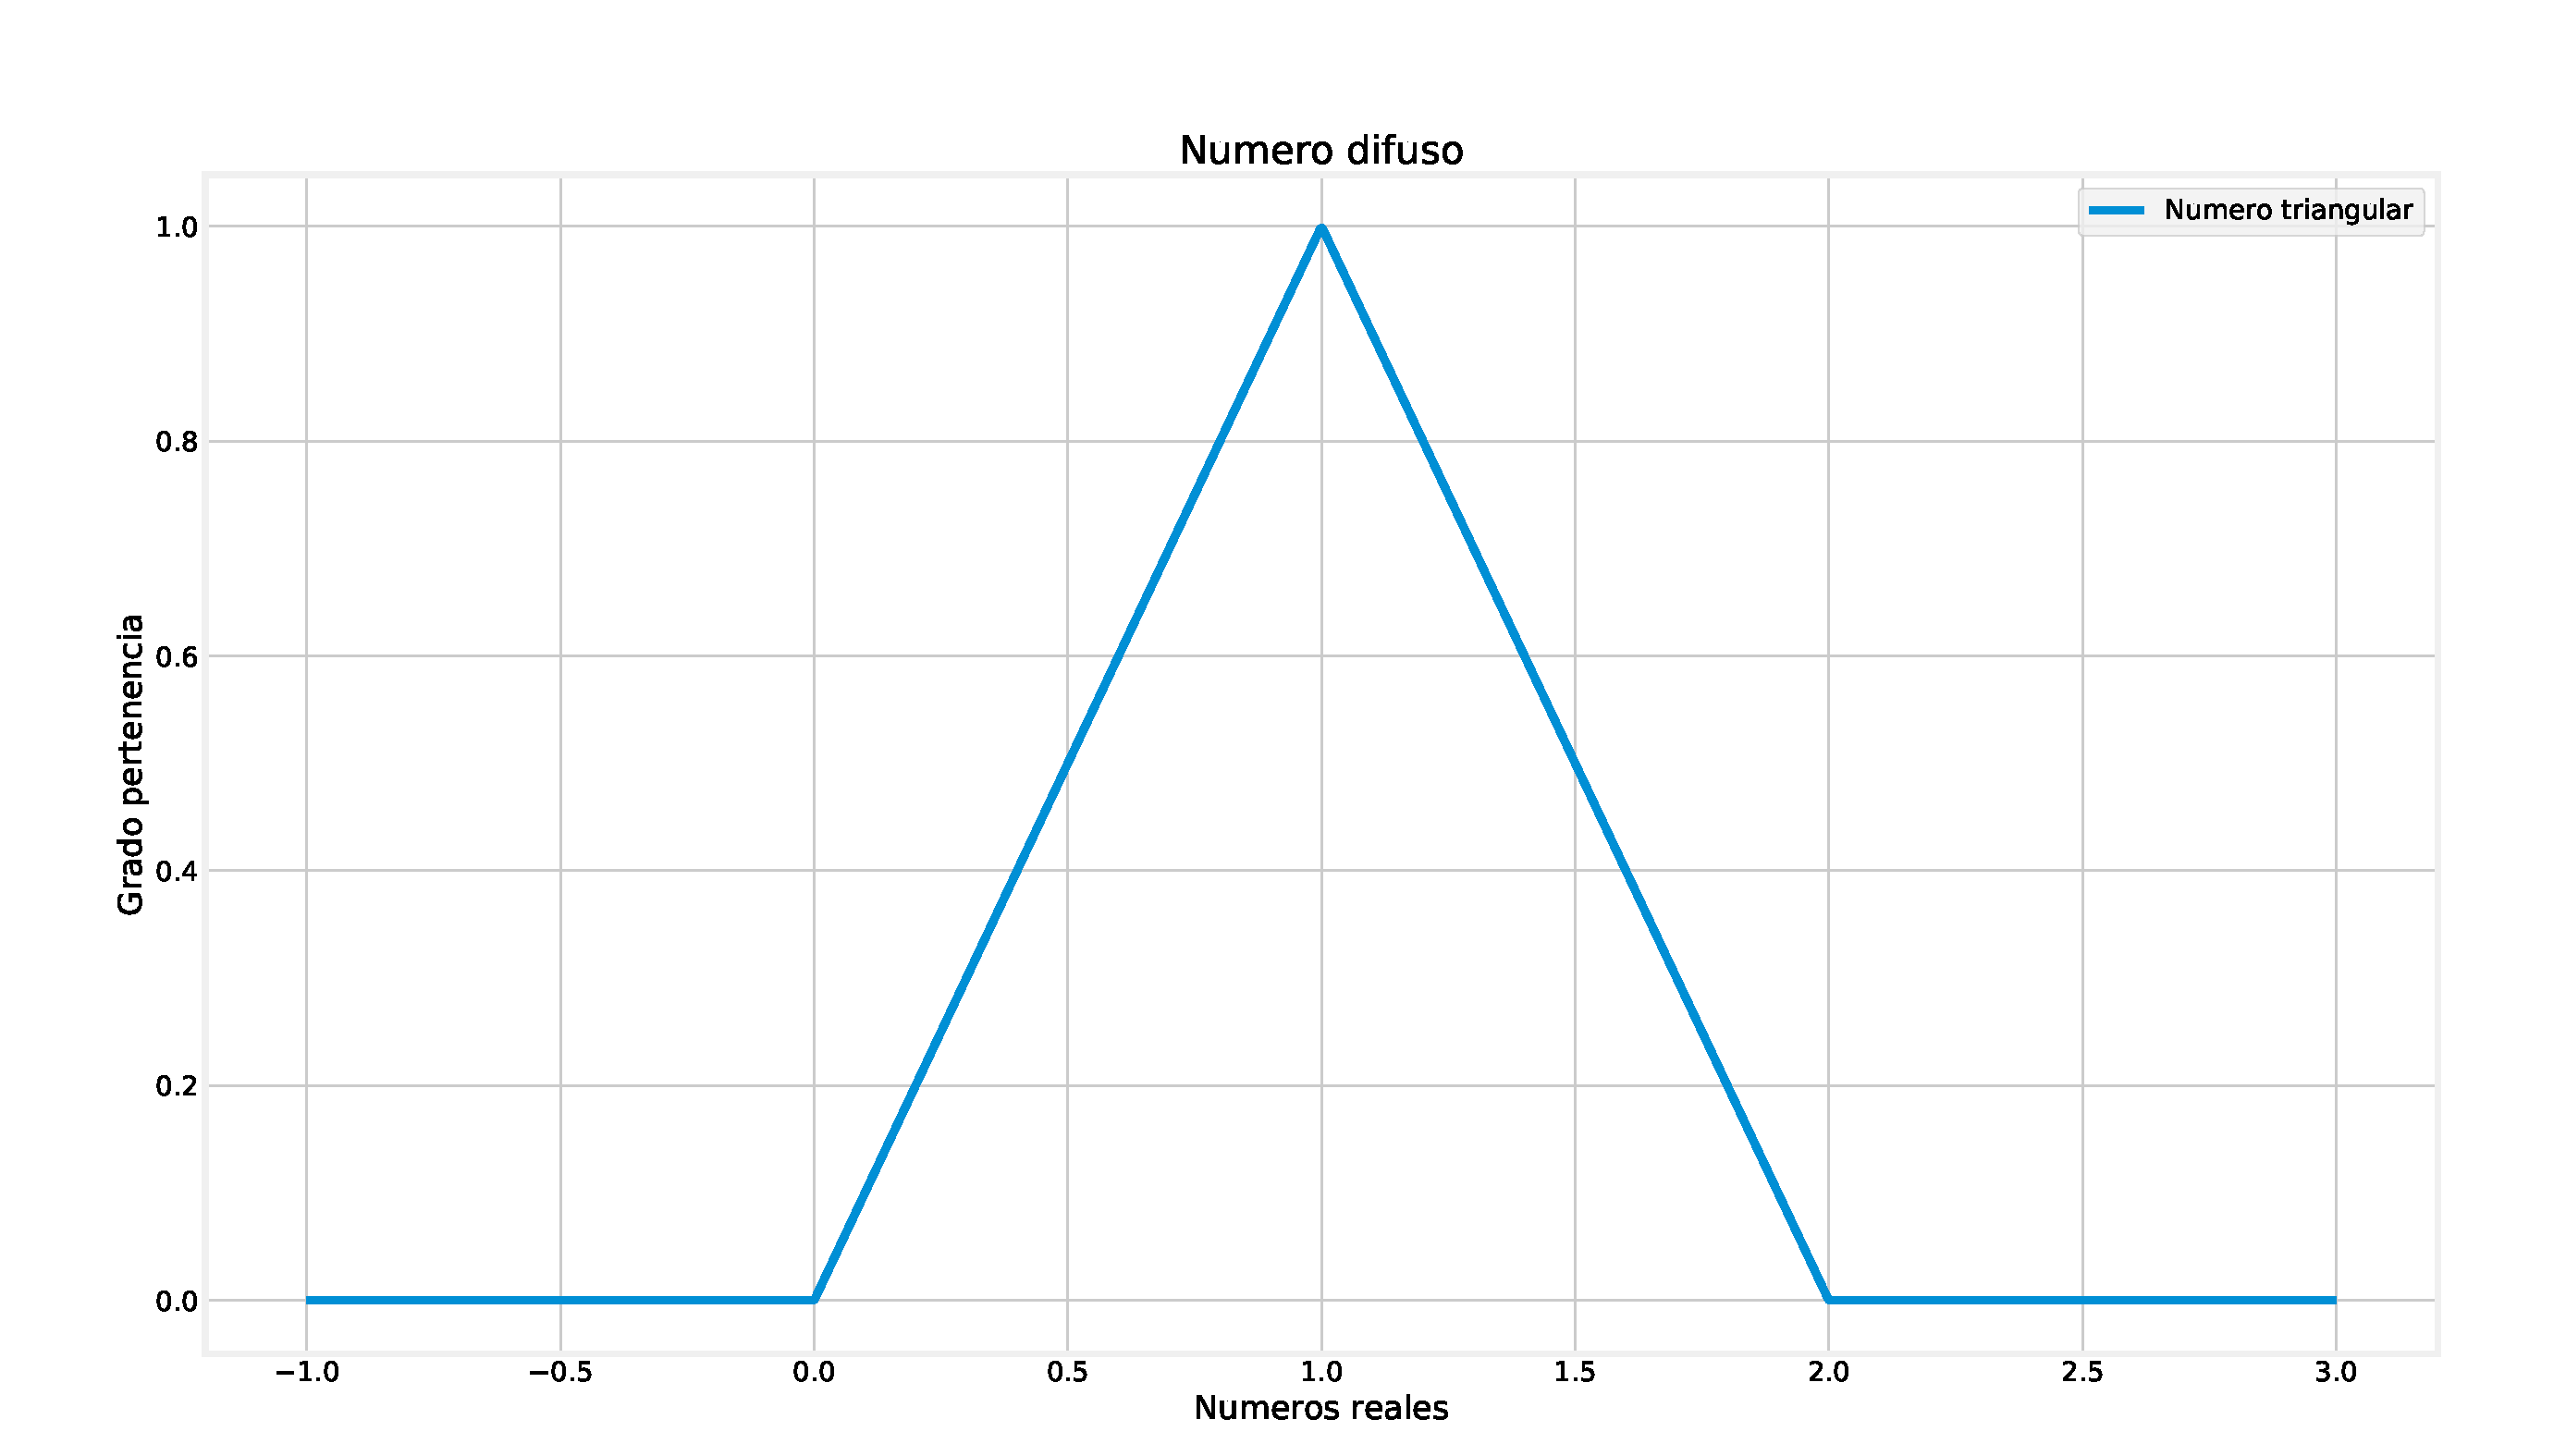
\includegraphics[width=\textwidth]{grafica_triangular}}
      \caption{Ejemplo de número triangular}
      \label{fig:numero_difuso}
    \end{figure}
    
  \end{ejemplo}


  \section{Principio de extensión de Zadeh}
  Estaría bien que dado un conjunto difuso, y una función clásica, fuese posible obtener una función difusa, para esto, se introduce el principio de extensión de Zadeh.

  \begin{definicion}[Principio de extensión de Zadeh]
  	\label{def:zadeh}
    Sean $\mathbb{U}$ y $\mathbb{V}$ dos conjuntos de universos, y sea $f: \mathbb{U} \longrightarrow \mathbb{V}$ una función clásica. Sea define el principio de extensión de Zadeh para todo conjunto difuso $A$ en $\mathbb{U}$ con $\mu_A$ su función de pertenencia, de manera que $\hat{f}(A)$ en $\mathbb{V}$ y su función de pertenencia viene dada por:
    
    $$
    \mu_{\hat{f}(A)}=\left\{
    \begin{array}{ccc}
      \sup_{x\in f^{-1}(y)} \mu_A(x) & si & f^{-1}(y)\neq\emptyset\\
      0 & si & f^{-1}=\emptyset
    \end{array}
    \right.
    $$
  \end{definicion}


  Se puede observar, que si la función es inyectiva, la función de pertenencia se simplificaría:
  $$
  \mu_{\hat{f}(A)}=\left\{
  \begin{array}{ccc}
    \mu_A(f^{-1}(y)) & si & f^{-1}(y)\neq\emptyset\\
    0 & si & f^{-1}=\emptyset
  \end{array}
  \right.
  $$

  \subsection{Teoremas de continuidad}
  Sería ideal que no importase el orden con el que se obtienen los $\alpha$-corte de la imagen de una función mediante el principio de extensión de Zadeh, y esto lo asegura el siguiente teorema.

  \begin{teorema}
  	\label{teorema:contfuzzy}
    Sea $f : \mathbb{R}^n \longrightarrow \mathbb{R}^m$ una función.
    \begin{enumerate}
    \item Si $f$ es sobreyectiva, entonces $[\hat{f}(A)]_\alpha = f([A]_\alpha)$ si y sólo si $\sup\{\mu_A(x) : x \in f^{-1}(y)\}$ para todo $y \in \mathbb{R}^m$
    \item Si $f$ es continua, entonces $\hat{f} : \mathcal{F}_\mathcal{H}(\mathbb{R}^n) \longrightarrow \mathcal{F}_\mathcal{H}(\mathbb{R}^n)$ está bien definido, y además,  
      $$[\hat{f}(A)]_\alpha = f([A]_\alpha)$$
      para todo $\alpha \in [0, 1]$
    \end{enumerate}
  \end{teorema}

  La primera implicación es clara por la definición de principio de extensión de Zadeh, para la segunda implicación se introduce un teorema más general:


  \begin{teorema}
    Sean $\mathbb{U}$ y $\mathbb{V}$ unos espacios de Haussdorf, y sea $f: \mathbb{U} \longrightarrow \mathbb{V}$ una función. Si $f$ es continua, entonces  $\hat{f} : \mathcal{F}_\mathcal{H}(\IR^n) \longrightarrow \mathcal{F}_\mathcal{H}(\IR^n)$ está bien definida y $$[\hat{f}(A)]_\alpha = f([A]_\alpha)$$
    para todo $\alpha \in [0, 1]$
  \end{teorema}

  \begin{proof}
    Por la definición del principio de Zadeh, se tiene que $\hat{f}(A)$ es un subconjunto difuso de $\mathbb{V}$. \\
    Para probar que $\hat{f} : \mathcal{F}_\mathcal{H}(\IR^n) \longrightarrow \mathcal{F}_\mathcal{H}(\IR^n)$ hay que ver que todos los $\alpha-corte$ $[\hat{f}(A)]_\alpha$ son no vacíos, compactos en $\mathbb{V}$. \\
    Dado que $f$ es continua por hipótesis, la imagen de compactos, son compactos, por tanto, sólo hay que probar $[\hat{f}(A)]_\alpha = f([A]_\alpha)$. \\
    Se procede por doble inclusión.
    
    \begin{itemize}
    \item $[\hat{f}(A)]_\alpha \subset f([A]_\alpha)$. Sea $\mathcal{A} \in \mathcal{F}_\mathcal{H}(\IU)$ y $y \in f([A]_\alpha)$. Por tanto, existe al menos un $x \in [A]_\alpha$ tal que $f(x)=y$. Por el principio de extensión de Zadeh, tenemos $\mu_{\hat{f}(A)}(y)=\sup_{x\in f^{-1}(y)} \mu_A(x) \geq \alpha$. De donde, $y \in [\hat{f}(\mathcal{A})_\alpha]$
    \item Por otro lado, hay que ver que $[\hat{f}(A)]_\alpha \supset f([A]_\alpha)$. Dado que $\mathbb{V}$ y $\mathbb{U}$ son espacios de Haussdorf, un punto $y \in \mathbb{V}$ es cerrado. Y además, dado que $f$ es continua, $f^{-1}(y)$ es cerrado. Dado que $[A]_0$ es compacto, ya que es la clausura, la intersección de compactos también es compactos, por tanto $f^{-1}(y) \cap [A]_0$ es compacto. Para $\alpha>0$, sea $y \in [\hat{f}(A)]_\alpha$. Entonces $\mu_{\hat{f}(A)}(y)=\sup_{x\in f^{-1}(y)} \mu_A(x) \geq \alpha>0$, y además, existe un $x\in f^{-1}(y)$ tal que $f^{-1}(y) \cap [A]_0 \neq \emptyset$
    \end{itemize}
    Finalmente, debido a que $\mu_A(x)$ es continúa por la derecha, y $f^{-1}(y) \cap [A]_0$ es compacto, existe un $x \in f^{-1}(y) \cap [A]_0$ con $\mu_{\hat{f}(\mathcal{A})}(y)=\mu_{\mathcal{A}}(x) \geq \alpha$. Esto es porque $y=f(x)$ para algún $x \in [A]_\alpha$.
    
    Para $\alpha=0$, se tiene:
    
    $$
    \bigcup_{\alpha \in (0, 1]} [\hat{f}(\mathcal{A})]_\alpha = \bigcup_{\alpha \in (0, 1]} f([\mathcal{A}]_\alpha) \subset f([\mathcal{A}]_0).
	$$
	
	Dado que $f([\mathcal{A}]_0)$ es cerrado:
	
	$$
	[\hat{f}(\mathcal{A})]_0 = cl\left( \bigcup_{\alpha \in (0, 1]} [\hat{f}(\mathcal{A})]_\alpha  \right) = cl\left(\bigcup_{\alpha \in (0, 1]} f([\mathcal{A}]_\alpha) \right)	\subset f([\mathcal{A}]_0).
	    $$
	    
	    Y por la doble inclusión anterior, se tiene que $[\hat{f}(\mathcal{A})]_\alpha \subset f([\mathcal{A}]_\alpha)$ para todo $\alpha \in [0, 1]$
  \end{proof}


  \section{Aritmética difusa}
  El siguiente paso \textbf{para poder construir métodos numéricos es necesario definir las operaciones aritméticas básicas} entre conjuntos difusos.\\
  La definiciones de \textbf{estas operaciones son bastante naturales}, pero pueden ocasionar algunos problemas en ciertos escenarios.\\
  Debido a la equivalencia entre trabajar con conjuntos difusos, y sus $\alpha-corte$, se centrará en dar todas las operaciones en términos de $\alpha-cortes$.\\
  En primer lugar, \textbf{se verá la definición habitual de aritmética en teoría de conjuntos clásicos.}

  \subsection{Aritmética en conjuntos clásicos}
  Sean $A, B$ dos conjuntos entonces:
  \begin{itemize}
  \item $A+B=\{a+b : a \in A, b\in B\}$
  \item $A - B =\{a - b : a \in A, b\in B\}$
  \item $A * B =\{ab : a \in A, b\in B\}$
  \item $A / B =\{a/b : a \in A, b\in B\}$
  \end{itemize}

  Una vez recordados los conceptos básicos de aritmética en conjuntos clásicos, se va a generalizar para conjuntos difusos.

  \subsection{Aritmética en conjuntos difusos}
  Sean $\mu_A, \mu_B$ dos funciones de pertenencia y sea $\odot \in \{+, -, \cdot, \div\}$ se define la función de pertenencia de la operación aritmética como:
  $$
  \mu_{A \odot B}(x) = \sup_{a \odot b = c} \min\{\mu_A(a), \mu_B(b)\}
  $$
  Y dado que \textbf{las operaciones aritméticas son funciones continuas}, es equivalente trabajar con los $\alpha-corte$, \textbf{aplicando el principio de extensión de Zadeh tenemos:}

  Sean $A$ y $B$ dos números difusos con $\alpha-corte$ dados por $[A]_\alpha=[a_\alpha^-, a_\alpha^+]$ y $[B]_\alpha=[b_\alpha^-, b_\alpha^+]$, se puede definir entonces las operaciones aritméticas como:

  $$
  [A+B]_\alpha = [a_\alpha^- + b_\alpha^-, a_\alpha^+ + b_\alpha^+]
  $$

  $$
  [A-B]_\alpha = [a_\alpha^- - a_\alpha^+, a_\alpha^+ - b_\alpha^-]
  $$

  $$
  [A \cdot B]_\alpha = \left[ \min_{s, r \in \{-, +\}} a_\alpha^s \cdot b_\alpha^r, \max_{s, r \in \{-, +\}} a_\alpha^s \cdot b_\alpha^r\right]
  $$

  $$
  [A \div B]_\alpha = \left[ \min_{s, r \in \{-, +\}} \frac{a_\alpha^s}{b_\alpha^r}, \max_{s, r \in \{-, +\}} \frac{a_\alpha^s}{b_\alpha^r}\right]
  $$

  \subsubsection{Problemas al definir estas operaciones aritméticas}
  El objetivo final es \textbf{definir la diferencial de una función}, para funciones escalares de una sola variable se define la diferencial como:
  $$
  \lim\limits_{h\rightarrow 0^+} \frac{f(x+h) - f(x)}{h}
  $$
  Se considera ahora una función $f(x)=A\in \mathcal{F}_\mathcal{H}(\IU)$, donde $A$ es un número difuso constante. \\
  $$f(x+h) - f(x)=[A-A]$$
  Sean $[A]_\alpha$ los $\alpha-cortes$ de $A$ entonces:
  $$
  [A-A]_\alpha = [a_\alpha^- - a_\alpha^+, a_\alpha^+ - a_\alpha^-]
  $$
  Si $A\neq 0$ se tiene que $[A-A]_\alpha \neq 0$, por tanto al dividir por $h \rightarrow 0$, tenemos una indeterminación, de donde, tal y \textbf{como se ha definido las operaciones aritméticas para los conjuntos difusos no estarían definidas las derivadas de funciones constantes}, y esto, es un problema. \\
  Necesitamos definir \textbf{un nuevo concepto de diferencia}, que para ello, \textbf{se introduce la diferencia de Hukuhara.}

  \subsection{Hukuhara y diferencia generalizada} \label{def:hukukara}
  Debido al problema especificado en la sección anterior, \textbf{se necesita definir una operación resta que cumpla que $A-A=\{0\}$}, Hukuhara dio una definición de resta que soluciona el problema expuesto en la sección anterior.

  \begin{definicion}
    Dados dos números difusos $A, B \in \mathcal{F}_\mathcal{C}\IR$ la \textbf{diferencia de Hukuhara (H-Diferencia)} se define como $A \circleddash_H B = C$ donde $C$ es el número difuso que cumple $A=B+C$, si existe.
  \end{definicion}

  \begin{observacion}
    Sean $A, B, C \in \mathcal{F}_\mathcal{C}\IR$ se consideran sus $\alpha - cortes$, por tanto $[A]_\alpha = [a^-_\alpha, a^+_\alpha]$, $[B]_\alpha = [b^-_\alpha, b^+_\alpha]$ y $[C]_\alpha = [c^-_\alpha, c^+_\alpha]$. \\
    De donde,
    $$
    [a^-_\alpha, a^+_\alpha] = [b^-_\alpha + c^-_\alpha, b^+_\alpha + c^+_\alpha]
    $$
    Por tanto, 
    $$
    [A \circleddash_H B]_\alpha = [a_\alpha^- - b_\alpha^-, a_\alpha^+ - b_\alpha^+]
    $$
  \end{observacion}
  Con esta observación es fácil ver que la H-Diferencia cumple que $A-A=\{0\}$
 
  Se pueden definir otras diferencias que mejoran el concepto anterior:
  
  \begin{definicion}[Diferencia de Hukuhara generalizada]
  	Dado dos números difusos $A, B \in \mathcal{F}_\mathcal{C}\IR$ se define la diferencia generalizada de Hukuhara (gH-diferencia) $A\circleddash_{gH}B=C$ donde $C$ es un número difuso que existe y cumple una de las siguientes condiciones:
  	
  	\begin{enumerate}
  		\item $A=B+C$ 
  		\item $B=A-C$
  	\end{enumerate}
  \end{definicion}

  \begin{definicion}[Diferencia generalizada]
	Dado dos números difusos $A, B \in \mathcal{F}_\mathcal{C}\IR$ se define la diferencia generalizada (g-diferencia) $A\circleddash_{g}B=C$ donde $C$ es un número difuso que existe y tiene los siguientes $\alpha$-cortes:
	\[
		[A \circleddash_{g} B]_\alpha = cl \bigcup_{\beta \geq \alpha} ([A]_\beta \circleddash_{gH} [B]_\alpha), \forall \alpha \in [0, 1]
	\]
  \end{definicion}

  \section{Interactividad}
  El principio de extensión de Zadeh se puede aplicar a funciones de distinto número de argumentos. Los ejemplos más simples podrían ser la suma, la resta, la multiplicación y la división de números difusos. Esta situación es más compleja, debido a que hay que tener en cuenta las estructuras entre los distintos argumentos. Esta dependencia mutua entre los distintos conjuntos difusos, viene dada por una función de pertenencia común denominada \textbf{función de pertenencia conjunta}. En términos de conjuntos difusos, esta dependencia se llama interactividad.

  \begin{definicion}[Interactividad, función de pertenencia conjunta]
    Sea $\hat{a} \in \mathcal{F}(V)$ y sea $\hat{b} \in \mathcal{F}(W)$. Entonces la interactividad de $\hat{a}$ y $\hat{b}$ se define por la función de pertenencia conjunta: $\mu_{\hat{a}, \hat{b}} : V \times W \rightarrow [0, 1]$
  \end{definicion}
  Para calcular las funciones de pertenencia marginales, simplemente hay que aplicar el principio de extensión de Zadeh:

  \begin{definicion}[Función marginal de una función de pertencia conjunta]
    Se define la función de pertenencia marginal respecto $a$ como:
    \[
    \mu_a(a) = \sup\lim\limits_{b \in W} \mu_{\hat{a}, \hat{b}} (a, b)
    \]
  \end{definicion}

  Se suele suponer no interactividad al trabajar con varios conjuntos difusos, esto es;

  \begin{definicion}[No interactivos o independientes]
    Dos conjuntos difusos $\hat{a} \in \mathcal{F}(V)$ y $\hat{b} \in \mathcal{F}(W)$ se dicen que son no interactivos, o independientes si $\mu_{\hat{a}, \hat{b}} = \min(\mu_{\hat{a}}(a), \mu_{\hat{b}}(b))$
  \end{definicion}

  \begin{ejemplo}
    En el caso de conjuntos no interactivos, se escriben las operaciones aritméticas de los conjuntos difusos de la siguiente manera:

    \[
      [\hat{a} + \hat{b}]_\alpha = [[\hat{a}^-_\alpha + [\hat{b}]_\alpha^-, [\hat{a}]^+_\alpha + [\hat{b}]_\alpha^+]
        \]

        \[
          [\hat{a} - \hat{b}]_\alpha = [[\hat{a}^-_\alpha - [\hat{b}]_\alpha^-, [\hat{a}]^+_\alpha - [\hat{b}]_\alpha^+]
            \]

            \[
              [\hat{a} * \hat{b}]_\alpha = \max\{ [\hat{a}]_\alpha^i [\hat{b}]^j_\alpha \}, i, j \in \{+, -\}
              \]

              \[
                [\hat{a} / \hat{b}]_\alpha = \max\{ [\hat{a}]_\alpha^i / [\hat{b}]^j_\alpha \}, i, j \in \{+, -\}
                \]
  \end{ejemplo}

  \section{Métrica en conjuntos difusos}
  En esta sección se va a generalizar la definición de espacio métrico a conjuntos difusos, y vamos a dar algunos resultados importantes. Todas las demostraciones de esta sección pueden encontrarse en \cite{apuntesfuzzy}. Se va a ver en primer lugar el concepto de métrica:

  \begin{definicion}[Pseudométrica]
    Sean $A$ y $B$ dos subconjuntos de un espacio métrico $\IU$ compactos. Entonces se define la pseudométrica como:
    \[
    \rho(A, B) = \sup\limits_{a \in A} d(a, B)
    \]
    Donde:
    \[
    d(a, B) = \inf\limits_{b \in B} ||a-b||
    \]
    es la separación de Haussdorf
  \end{definicion}

  \begin{definicion}[Métrica de Pompeiu-Hausdorff]
    \label{def:metricadifusa}
    Sean $A$ y $B$ dos conjuntos difusos en $\IU$, un espacio métrico. La métrica de Pompeiu-Hausdorff, denotada por $d_\infty$ se define:
    \[
    d_\infty(A, B) = \sup\limits_{\alpha \in [0, 1]} \max\{\rho([A]_\alpha, [B]_\alpha), \rho([B]_\alpha,  [A]_\alpha)\}
    \]
    
    Si $A$ y $B$ fueran números difusos, tendríamos:
    \[
    d_\infty(A, B) = \sup\limits_{\alpha \in [0, 1]} \max\{|a_\alpha^- - b_\alpha^-|, |a_\alpha^+ - b_\alpha^+|\}
    \]
  \end{definicion}

  \begin{teorema}[\cite{banachfuzzy}]
    \label{teorema:banach}
    El espacio de los números difusos, con la métrica $d_\infty$ es un espacio de Banach.
  \end{teorema}

  \section{Funciones difusas}
  En la literatura sobre funciones difusas existen dos definiciones para referirnos a funciones difusas, originalmente Dubois y Prade (1980) definieron los siguientes conceptos:

  \begin{definicion}[Funciones definidas en conjuntos difusos]
    \label{def:fizzusetvaluedfunc} Se dice que una función \textbf{$F$ es una función definida en un conjunto difuso} si:
    \begin{enumerate}
    \item $dom ~ F \subset \IR$
    \item $Im ~ F \subset \mathcal{F}_\mathcal{H}(\IR^n)$
    \end{enumerate}
  \end{definicion}

  \begin{ejemplo}
    La función $f(x) = A x$ donde $A=[a, b]$ con $a, b \in \IR$, es una función definida en conjuntos difusos. Sus imágenes son intervalos.
  \end{ejemplo}

  \begin{ejemplo}
    La función $f(x) = A x$ donde $A=(a;b;c)$ con $a<b<c$, es una función definida en conjuntos difusos. Además, su imágenes son conjuntos números triangulares.
  \end{ejemplo}

  \iffalse
  \begin{definicion}[Ristra de funciones difusas]
    Definimos una ristra de funciones difusas como el subconjunto difuso del espacio de funciones. \\
    Para cada ristra de funciones difusas, podemos darle una función definida en un conjunto difuso. Para cada $F \in \mathcal{F}(E(I; \IR^n))$ donde $E(I, \IR^n)$ es una espacio de funciones de $I \subset \IR$ a $\IR^n$. Donde:
    \[
      [F(t)]_\alpha = [F]_\alpha(t) = \{f(t) : f \in [F]_\alpha\}
      \]
  \end{definicion}

  \begin{ejemplo}
    Consideramos $f_1, f_2$ y $f_3$ funciones continuas en el intervalo $A=[a, b]$. Y definimos el conjunto difuso $F \in \mathcal{F}(C([a, b]; \IR))$ tal que:
    \[
    \mu_F(f) = \left\{
    \begin{array}{ccc}
      \alpha & si & f = f_1 + \alpha(f_2 - f_1) \\
      \alpha & si & f = f_3 + \alpha(f_2 - f_3) \\
      0 & otro~caso & 
    \end{array}
    \right.
    \]
    
    Entonces, decimos que $F$ es una ristra de funciones difusas.
  \end{ejemplo}

  \fi

  \subsection{Continuidad de funciones difusas}
  Se introduce en primer lugar dos conceptos de continuidad sobre funciones reales que toman valores en subconjuntos reales. Y luego, usaremos esta misma idea para definir la continuidad sobre conjuntos difusos

  \begin{definicion}[Función sobre conjuntos continua]
    \label{def:funcioncontinua}
    Sea $F : \Omega \rightarrow \mathcal{P}(\IR^n)$, $\Omega \subset \IR^m$ se dice que $F$ es \textbf{semicontinua superiormente} en $t_0 \in \Omega$, si para todo $\varepsilon>0$ existe un $\delta>0$ tal que:
    \[
    \rho(F(t), F(t_0))<\varepsilon
    \]
    Si $||t-t_0||<\delta$ para $t \in \Omega$. \\
    Por otro lado, se dice que $F$  es \textbf{semicontinua inferiormente} en $t_0 \in \Omega$, si para todo $\varepsilon>0$ existe un $\delta>0$ tal que:
    \[
    \rho(F(t_0), F(t))<\varepsilon
    \]
    Si $||t-t_0||<\delta$ para $t \in \Omega$. \\
    Si una función es semicontinua superiormente e inferiormente, se dice que es \textbf{continua.}
  \end{definicion}

  \begin{definicion}[Función difusa continua]
    Sea $F : \Omega \rightarrow \mathcal{F}_\mathcal{H}(\IR^n)$, $\Omega \subset \IR^m$ se dice que $F$ es \textbf{semicontinua superiormente} en $t_0 \in \Omega$, si para todo $\varepsilon>0$ existe un $\delta>0$ tal que:
    \[
    \rho([F(t)]^\alpha, [F(t_0)]^\alpha)<\varepsilon
    \]
    Si $||t-t_0||<\delta$ para $t \in \Omega$, para todo $\alpha \in [0, 1]$. \\
    Por otro lado, se dice que $F$ es \textbf{semicontinua superiormente} en $t_0 \in \Omega$, si para todo $\varepsilon>0$ existe un $\delta>0$ tal que:
    \[
    \rho([F(t_0)]^\alpha, [F(t)]^\alpha)<\varepsilon
    \]
    Si $||t-t_0||<\delta$ para $t \in \Omega$, para todo $\alpha \in [0, 1]$. \\
    Si una función es semicontinua superiormente e inferiormente, se dice que es \textbf{continua.}
  \end{definicion}

  \iffalse
  \subsection{Representación gráfica de funciones difusas}
  En este sección se va a buscar una solución al problema de representar funciones difusas.

  Una representación gráfica de una función difusa podemos desear que cumpla lo siguiente:
  \begin{enumerate}
  \item El grado de pertenencia debe verse de forma intuitiva.
  \item Si nuestra función toma valores en $\IR^n$ y va $\mathcal{F}_\mathcal{H}(\IR^m)$, la gráfica debería de estar representada en $n+m+1$. Necesitamos una dimensión más debido a que los $\alpha$-corte son $m$-intervalos.
  \end{enumerate}

  \subsubsection{Gráfica de una función difusa}

  Siguiendo los puntos de la introducción, vamos a tratar de dar una solución a cada uno de los puntos:

  \begin{enumerate}
  \item El grado de pertenencia podemos representarlo usando colores. Fijamos un color inicial, que definiremos como $0$ y fijamos otro color final que definiremos como $1$. Todos los colores que hay entre el color inicial y final, representarán los grados de pertenencia. Por ejemplo, si tomamos como $0$ el color blanco $(255, 255, 255)$ y tomamos el color negro $(0, 0, 0)$ como color final, si queremos representar un valor con grado de pertenencia $\alpha$, deberíamos tomar el color: $(255(1-\alpha), 255(1-\alpha), 255(1-\alpha))$
    
  \item Por cada $x$ representamos una recta que contenga todos los valores que puede recorrer $f(x)$ y estos valores los pintamos según el grado de pertenencia especificado en el apartado anterior.
  \end{enumerate}
  \fi
